\documentclass{article}
\usepackage{tikz}
\usepackage{float} 
\usepackage{algorithm}
\usepackage{algpseudocode}

\title{Segment Trees in Algorithmic Problems}
\author{Piotr Szczepaniak}
\date{\today}

\begin{document}

\maketitle

\tableofcontents

\begin{abstract}
This document provides an overview of segment trees. In the first place
I will describe some algebraic topics which are necessary for better
understanding how and why segment trees works. This knowledge will be useful
for reading the rest of the paper where We will dive into different kinds of trees.
For each structure, I will explain how it work and how to apply it to problems.
Then, I will look at each structure's time complexity and space complexity.
\end{abstract}

\section{Foundations of Segment Trees}
A segment tree is a binary tree used for storing information about segments. 
To efficently retrieve or update informations about elements stored 
in segment tree we can perform various operations, the 
most common of which is the range query, range update or point update
(which is sipler case of range update). One of the examples of use can be maximum value of 
elements in given range or sum of elements in given range.

\begin{figure}[H]
    \centering
    
\begin{center}
    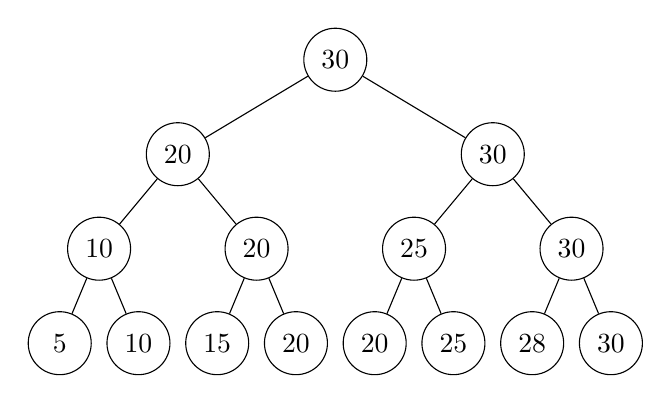
\begin{tikzpicture}[
      level distance=1.2cm,
      level 1/.style={sibling distance=4cm},
      level 2/.style={sibling distance=2cm},
      level 3/.style={sibling distance=1cm},
      every node/.style={draw,circle,minimum size=8mm,inner sep=1pt}
    ]
    
    % Root node with max value
    \node {30}
        child {node {20}
            child {node {10}
                child {node {5}}
                child {node {10}}
            }
            child {node {20}
                child {node {15}}
                child {node {20}}
            }
        }
        child {node {30}
            child {node {25}
                child {node {20}}
                child {node {25}}
            }
            child {node {30}
                child {node {28}}
                child {node {30}}
            }
        };
    
    \end{tikzpicture}
\end{center}
    \caption{Example of a segment tree with maximum value of elements in given range.}
    \label{fig:segment_tree}
\end{figure}

\subsection{Operation types}
To ilustrate use case of segment tree we will construct tree with max value on segment.
Let's say we are given an array \(A = [5, 10, 15, 20, 30, 25, 28, 20]\) of length \(n = 8\).
For now let's assume that the input array is of size \(n = 2^{k}\) where \(k\) is integer (for different
sizes of input we will fill input array with neutral elements (see section 2) to make it's length a power of 2).
The height of tree is \(h = \log{2}{n}\). Let's define \(dep(i)\) as depth of node i in our tree.
We can see that \(dep(root) = 0\) and \(dep(leaf) = h\).
We want to be able to perform the following operations:
\begin{itemize}
    \item \textbf{Build structure} \\
    We will create a segment tree from an array.
    To build a segment tree need to create a binary tree where each node will store the maximum value of elements in its subtree. \\
    \begin{algorithm}
    \caption{Build Segment Tree for Maximum on Segment (Iterative)}
    \begin{algorithmic}
        \Procedure{BuildTree}{arr, seg}
            \For{$i = 0$ \textbf{to} $n - 1$} \Comment{Fill leaves of the segment tree}
                \State $seg[n + i] \gets A[i]$
            \EndFor
            \For{$i = n - 1$ \textbf{downto} $1$} \Comment{Calculates nodes from bottom to top}
                \State $seg[i] \gets \max(seg[2 \times i], seg[2 \times i + 1])$
            \EndFor
        \EndProcedure
    \end{algorithmic}
\end{algorithm}

    This approach of building a segment tree gives us an array \(seg\) where
    \(seg[n, n*2 - 1]\) are values form input and value at 

    \item \textbf{Point update} \\
    Change the value of an element at a given index.
    \item \textbf{Range query} \\
    Find the sum of elements in a given range.
\end{itemize}



\subsection{Monoids}
A monoid \( (S, e, \ast) \) is a set equipped with an associative binary operation \( S \times S \to S \) and
an identity element \(e\). 
\begin{itemize}
    \item \textbf{Associativity} \\
    For all \( a, b, c \in S \), \( (a \ast b) \ast c = a \ast (b \ast c) \).
    \item \textbf{Identity element} \\
    There exists an element \( e \in S \) such that for all \( a \in S \), \( a \ast e = e \ast a = a \).
\end{itemize}


\end{document}